\placelogofalse
\begin{frame}{Applications: Topology Optimization}
\begin{columns}

  \column{0.31\linewidth}
  \centering
  \begin{center}
  \shadowimage[width=3.0cm]{giga_opt_paper.png}
  \vspace{0.5cm}
  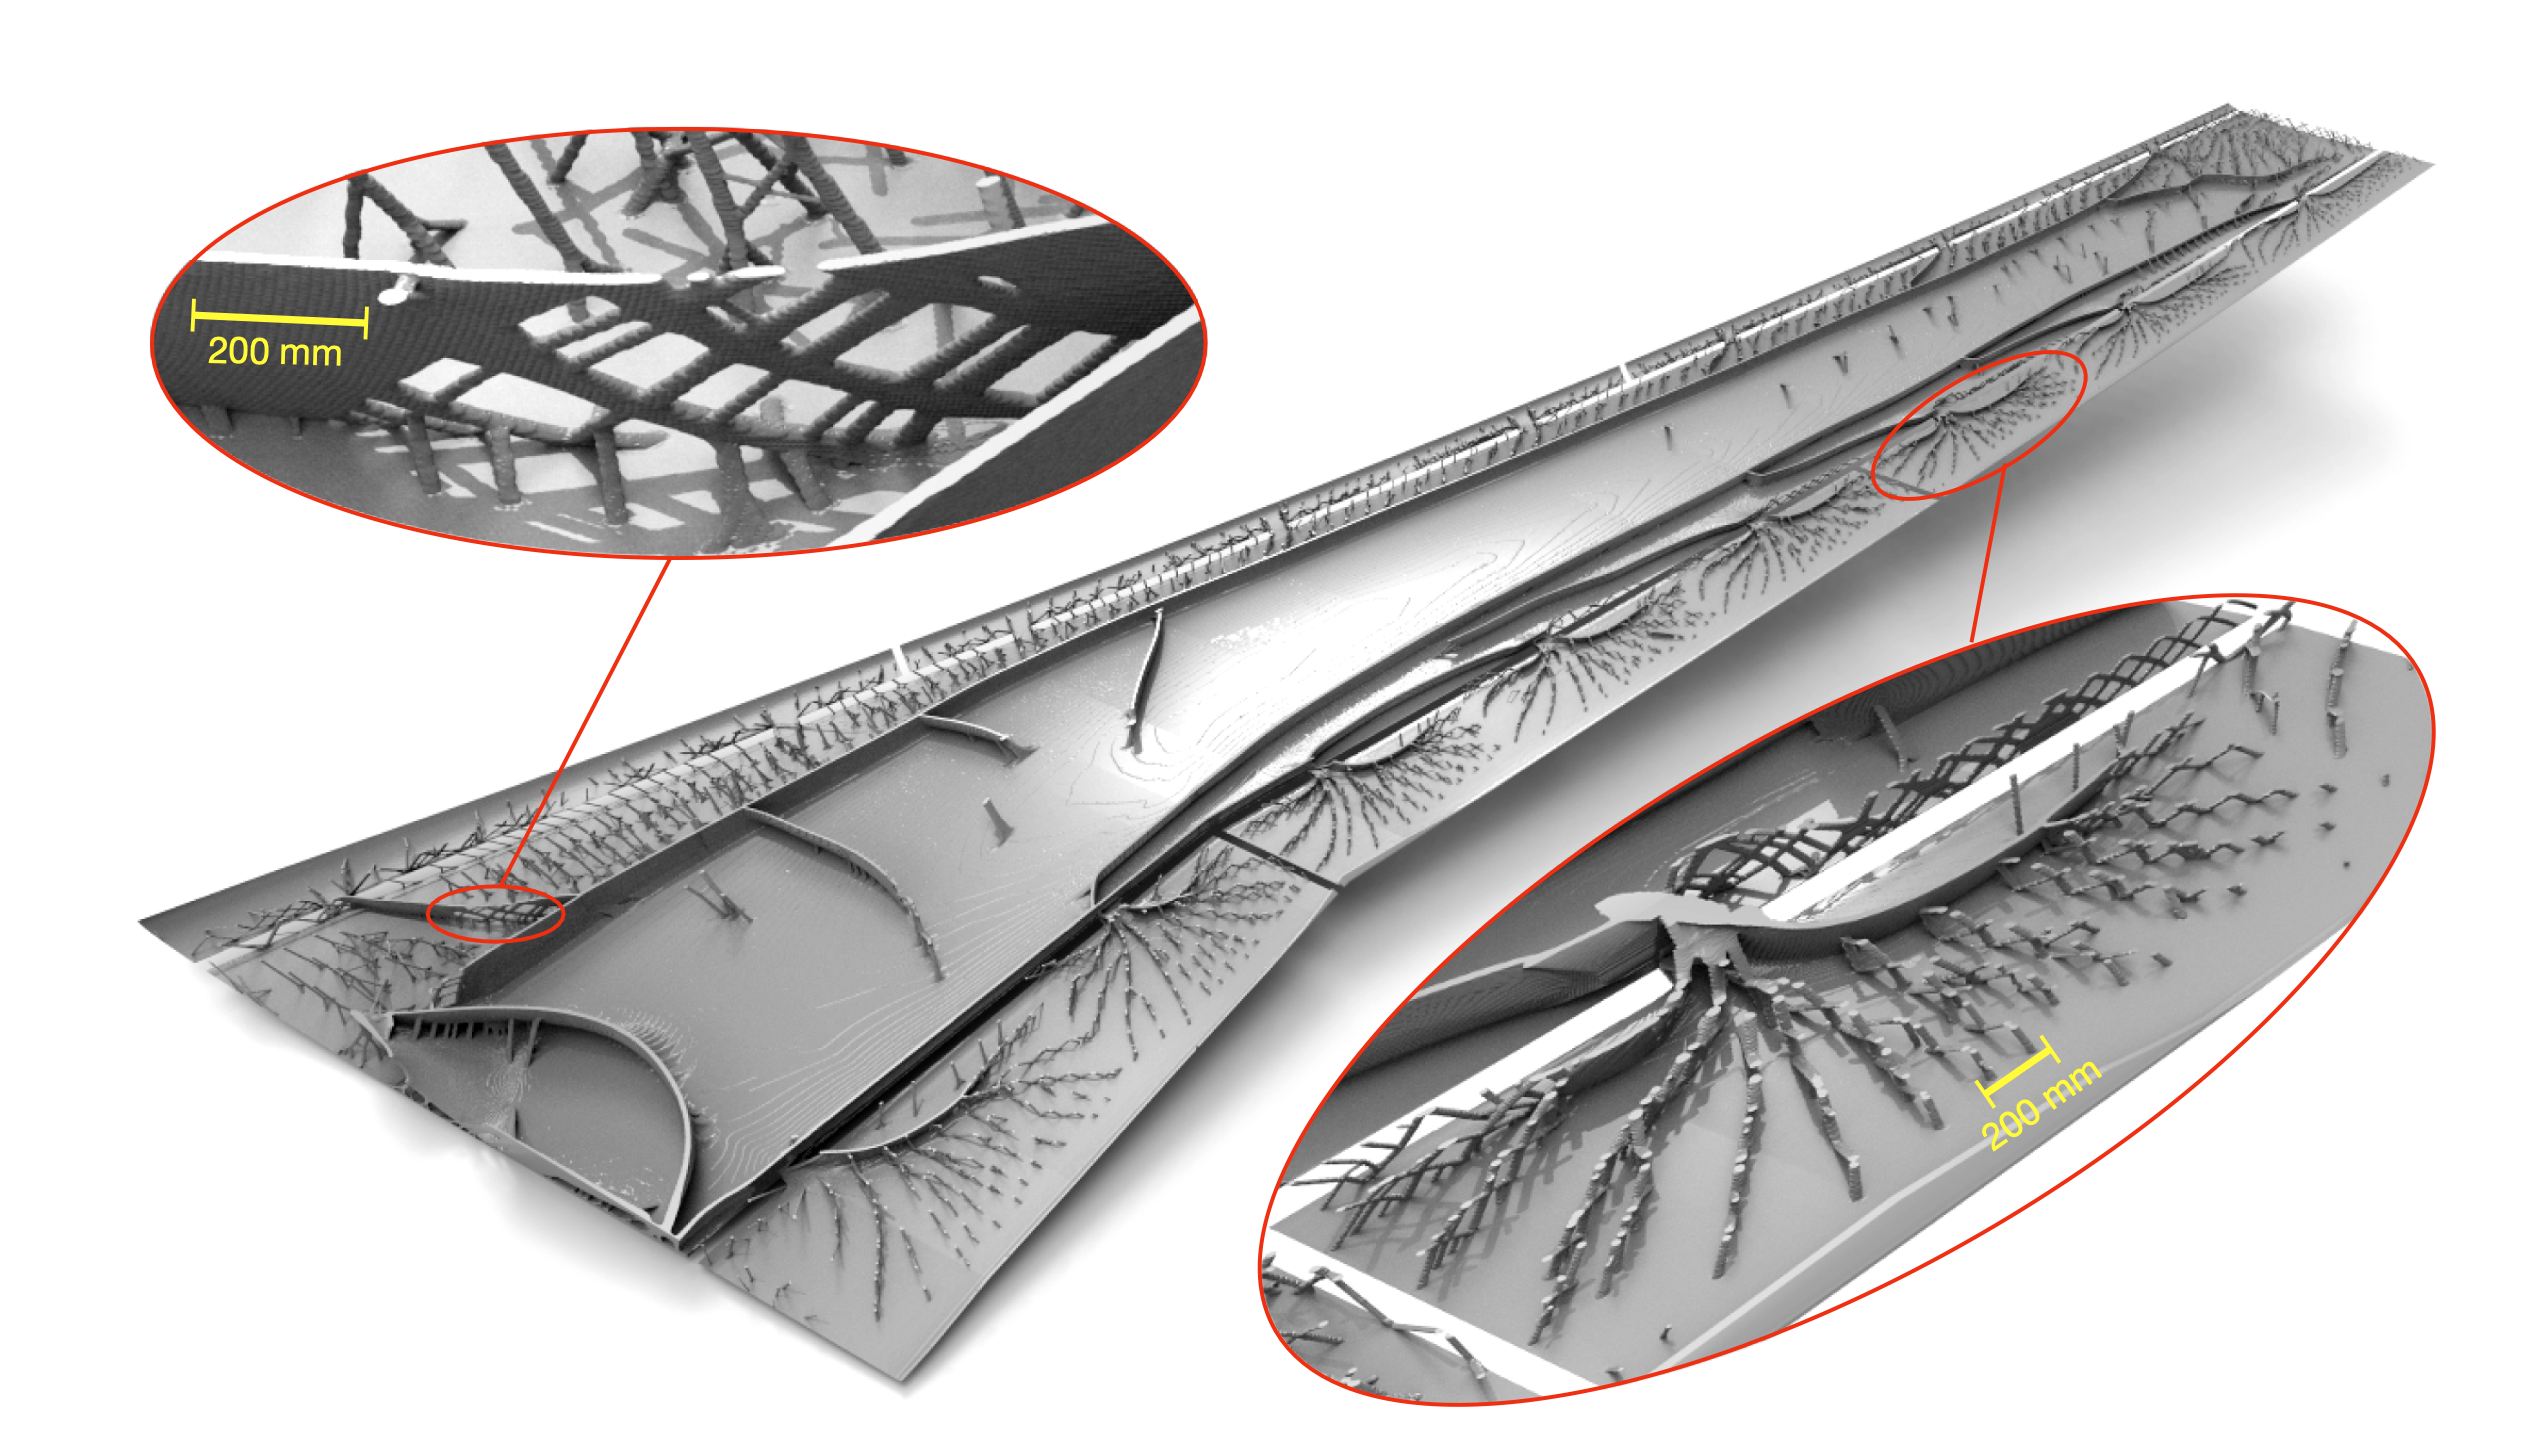
\includegraphics[width=3.0cm]{giga_opt_diagram.png}\\
  2017 \cite{Aage2017}
  \end{center}

  \column{0.31\linewidth}
  \centering
  \textbf{Giga-voxel Problems}
  \begin{outline}
  \1 $\approx 1$ Billion Active Voxels
  \1 1-5 day runtime
  \end{outline}
  \vspace{0.5cm}
  \textbf{$\leftarrow$ Prior SotA}
  \begin{outline}
  \1 8000 cores over many nodes
  \end{outline}
  \vspace{0.5cm}
  \textbf{Taichi Based $\rightarrow$}
  \begin{outline}
  \1 Single 14 core workstation  
  \end{outline}

  \column{0.31\linewidth}
  \centering
  \begin{center}
  \shadowimage[width=3.0cm]{top_opt_paper.png}
  \vspace{0.5cm}
  \shadowimage[width=3.0cm]{top_opt_02.png}
  2018 \cite{Liu2018}
  \end{center}
\end{columns}
\end{frame}
\placelogotrue

\placelogofalse
\begin{frame}{Applications: Differentiable Physics}
\begin{columns}
  \column{0.51\linewidth}
  \centering
  \begin{outline}
    \1 Soft Robotics
    \2 Difficult to design
    \2 Difficult to control
    \1 Simulation
    \2 Sparse representation 
    \2 Differentiable for learning / optimizing
  \end{outline}
  \vspace{0.5cm}
  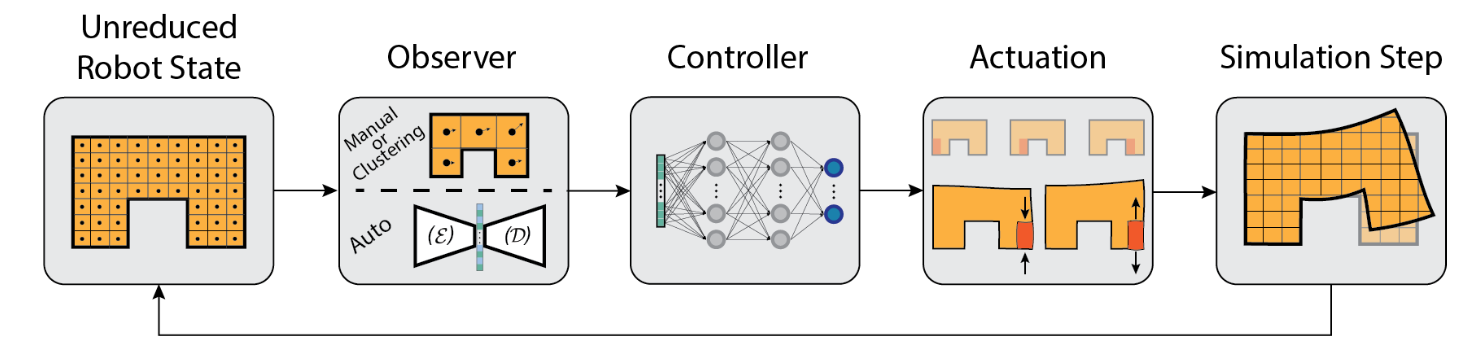
\includegraphics[width=6cm]{soft_robotics.png}

  \column{0.21\linewidth}
  \centering
  \begin{center}
  \shadowimage[width=2.5cm]{chain_queen_paper.png}
  \vspace{0.5cm}
  \includegraphics[width=2.5cm]{chain_queen_experiment.png}
  2019 \cite{Hu2019chainqueen}
  \end{center}

  \column{0.21\linewidth}
  \centering
  \begin{center}
  \shadowimage[width=2.5cm]{litlo_paper.png}
  \vspace{0.5cm}
  \shadowimage[width=2.0cm]{litlo_image.png}
  2019 \cite{Spielberg2019}
  \end{center}
\end{columns}
\end{frame}
\placelogotrue

\placelogofalse
\begin{frame}{Applications: Quantized Graphics}
\begin{columns}
  \column{0.48\linewidth}
  \begin{outline}
    \1 Decouple algorithms 
    from data representation
    \1 Lower memory requirements
    \2 8x Game of Life
    \2 1.5x Eulerian Fluid
    \2 1.7x Material point method
    \1 Leads to faster runtimes
  \end{outline}

  \column{0.48\linewidth}
  \centering
  \begin{center}
  \shadowimage[width=3.0cm]{quan_taichi_paper.png}
  2021 \cite{Hu2021} \\
  \vspace{0.3cm}
  \shadowimage[width=4.5cm]{quantized_demo.png}\\
  \end{center}
\end{columns}
\end{frame}
\placelogotrue
